\documentclass[compress]{beamer}
%,hyperref={pdfpagelabels=false}

\usepackage[ngerman,english]{babel}
\usepackage[T1]{fontenc}
\usepackage[latin1]{inputenc}
\usepackage{amsmath}
\usepackage{amsthm}
\usepackage{amsfonts}
\usepackage{helvet}
\usepackage{url}
\usepackage{listings}
\usepackage{xcolor}
\usepackage{xspace} % Abstand hinter Variablennamen
\usepackage{fix-cm}
%\usepackage[square, sort, numbers, authoryear]{natbib}

\usepackage{beamerthemeLEA2}

%\bibliographystyle{plainnat}

\newcommand{\N}       {\mathbb{N}}          % nat�rliche Zahlen
\newcommand{\Z}       {\mathbb{Z}}          % ganze Zahlen
\newcommand{\R}       {\mathbb{R}}          % reelle Zahlen
\newcommand{\Prob}    {\mathrm{P}}          % Wahrscheinlichkeit
\newcommand{\inter}   {\cap}                % Schnittmenge
\newcommand{\union}   {\cup}                % Vereinigung
\newcommand{\Oh}      {O}                   % O-Notation (Landau-Symbole)
\newcommand{\mycite}[1]{\textcolor{tumgreen}{[#1]}} 

\newenvironment{changemargin}[2]{% 
  \begin{list}{}{%
    \setlength{\topsep}{0pt}%
    \setlength{\leftmargin}{#1}%
    \setlength{\rightmargin}{#2}%
    \setlength{\listparindent}{\parindent}%
    \setlength{\itemindent}{\parindent}%
    \setlength{\parsep}{\parskip}%
  }%
  \item[]}{\end{list}}

\title{A Flexible Tool for Shape Analysis}
\subtitle{IDP Presentation}
\author{\href{emanuel.laude@in.tum.de}{Emanuel Laude}\\ \href{laehner@in.tum.de}{Zorah L\"ahner} } 
%\date{\today}
\date{January 16, 2015}
\institute{Technische Universit�t M�nchen}

% Inhaltsverzeichnis zu Begin von jedem Abschnitt einblenden?
%\AtBeginSection[]{
%  \begin{frame}
%    \frametitle{Outline}
%    \tableofcontents[currentsection]
%  \end{frame}
%}

\begin{document}

\begin{frame}
  \titlepage
\end{frame}

% Inhaltsverzeichnis
\begin{frame}
  \frametitle{Outline}
  \tableofcontents
\end{frame}

\section{Demo Time}

\section{Class Overview}

\begin{frame}
  \frametitle{Class Diagram: View}
  \begin{figure}[h]
	\centering
	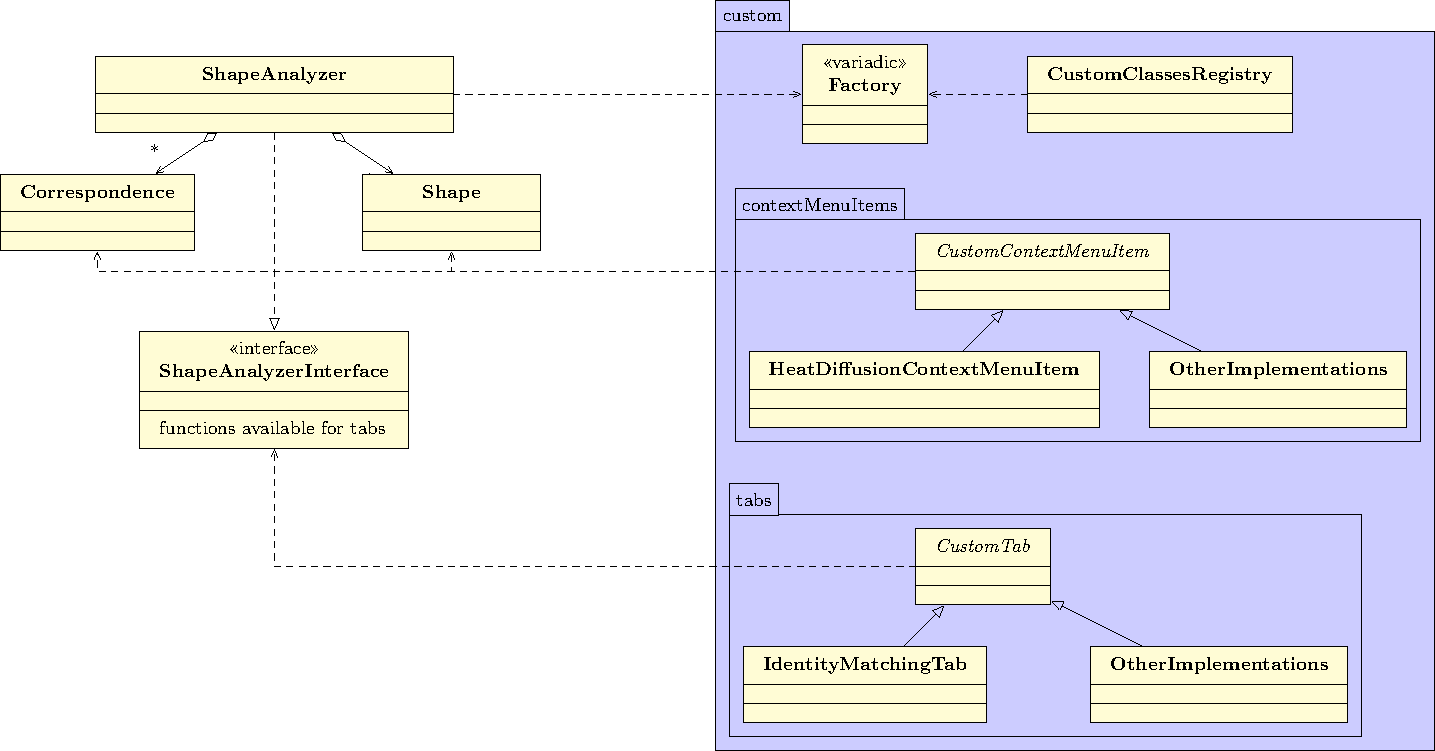
\includegraphics[width=\textwidth]{diagram.pdf}
\end{figure}
\end{frame}

\begin{frame}
  \frametitle{Class Diagram: Domain}
  \begin{figure}[h]
	\centering
	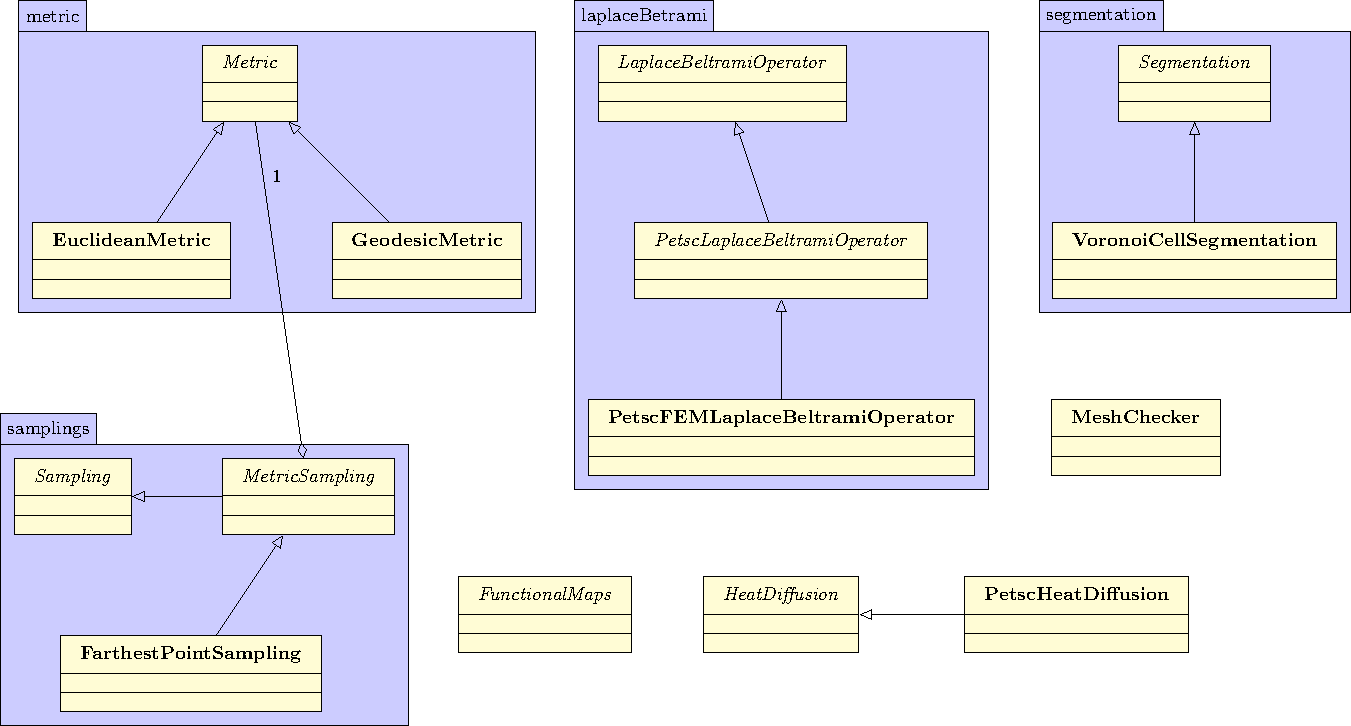
\includegraphics[width=\textwidth]{diagram2.pdf}
\end{figure}
\end{frame}

\section{Customs}

\begin{frame}[c]
  \frametitle{Customs}
  \begin{center}
  
  \huge CustomContextMenuItem 
  
  \vspace{1em}
  
  or 
  
  \vspace{1em}
  
  CustomTab?
  \end{center}
\end{frame}

\begin{frame}
  \frametitle{Example: VoronoiCellsContextMenuItem}
  
\end{frame}

\section{Demo Time: Functional Maps}

\begin{frame}
  \frametitle{Example:}
  
\end{frame}

\end{document}
